\section{Calibrazione}
Prima di procedere con le misure dei relativi esperimenti, abbiamo ritenuto necessario compiere una verifica della calibrazione dello strumento per ottenere risultati con maggiore precisione.
Abbiamo proceduto effettuando più volte il conteggio delle frange passanti per un riferimento scelto, per uno spostamento determinato \textit{d} del nonio pari a $20\,\mu m$.

I dati ottenuti per la determinazione di $d$ attraverso le diverse misurazioni sono riportati nella Tabella \ref{tabella 1}.

Facendo uso di \textsc{ROOT} ci è stato possibile effettuare un fit dei dati, dal quale abbiamo ricavato un nuovo valore di aspettazione, indicato nell'istogramma in Figura \ref{figura 3}.
\begin{figure}[h!]
    \centering
    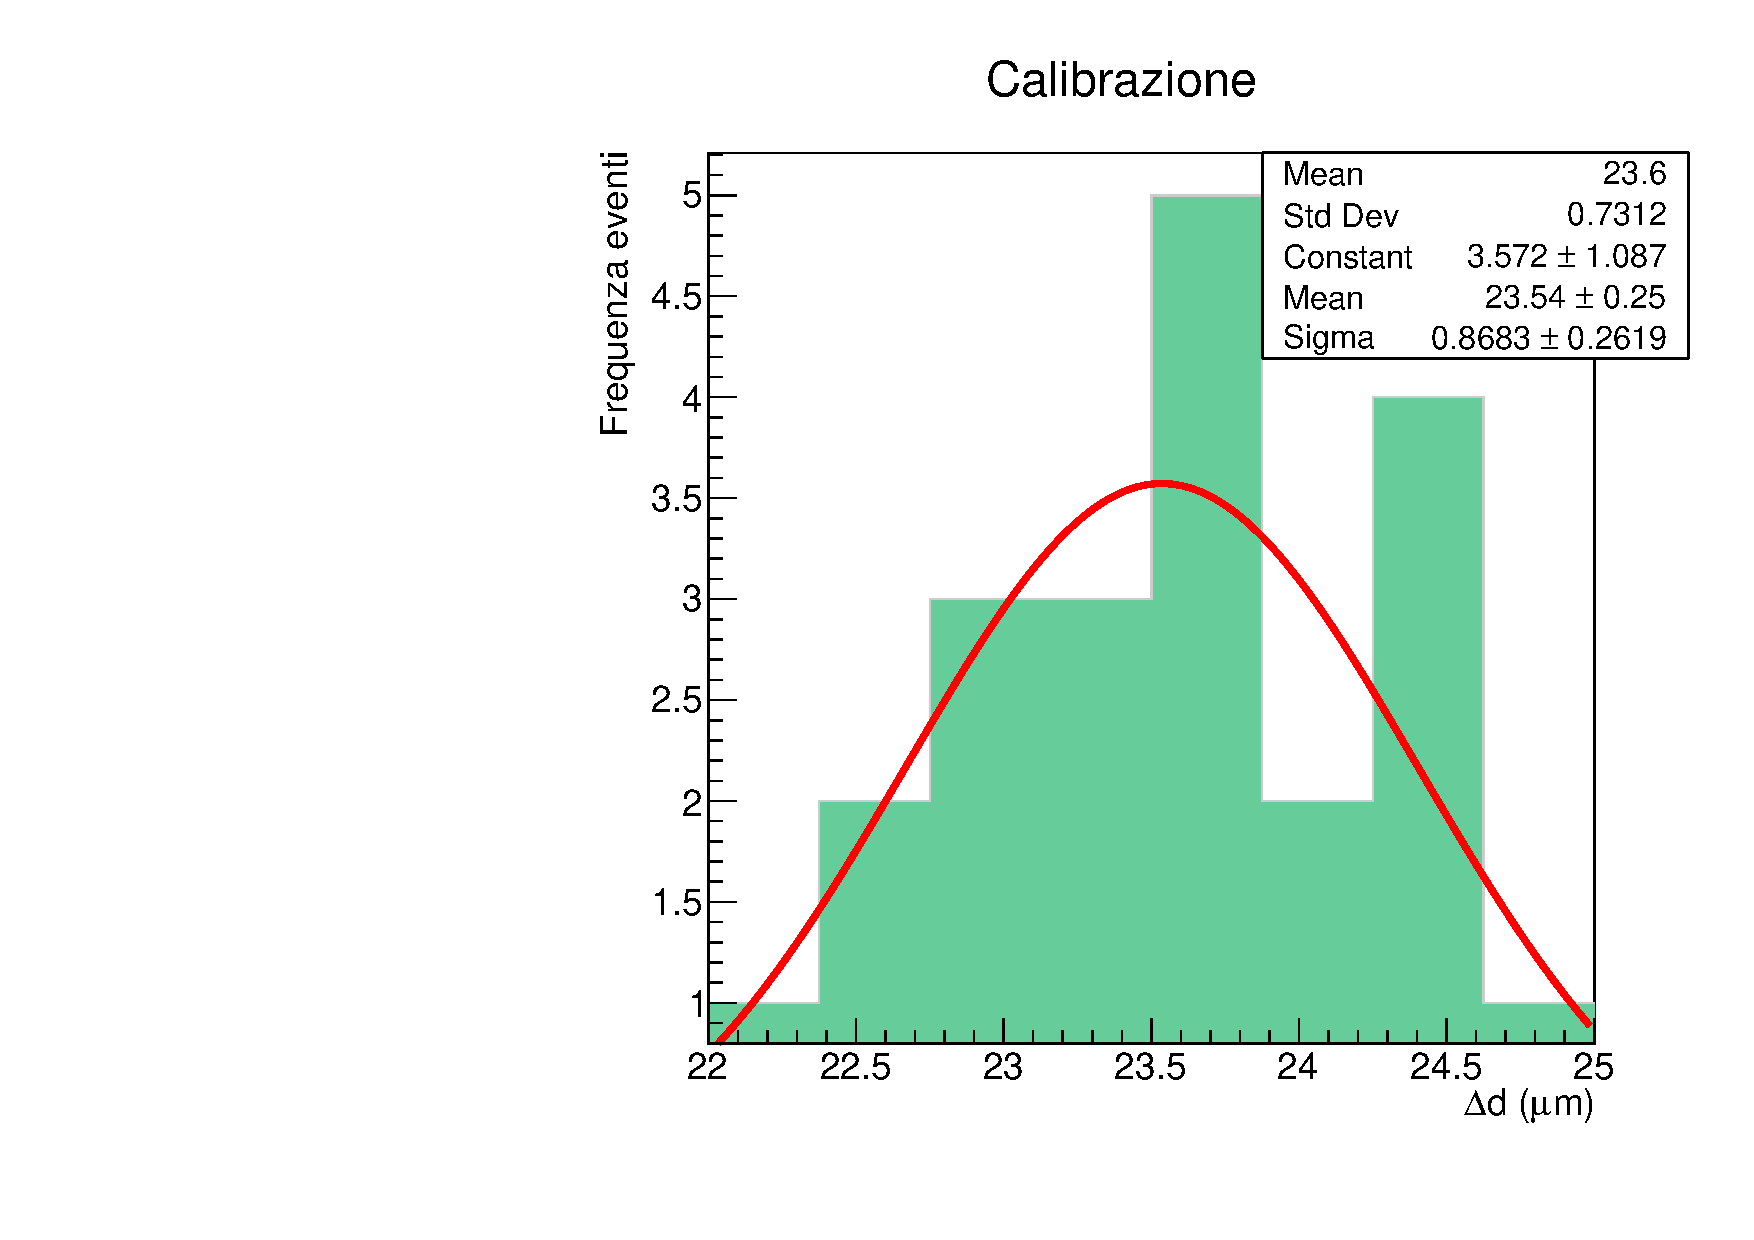
\includegraphics[scale=.35]{immagini/calibrazione nonnio.pdf}
    \caption{}
    \label{figura 3}
\end{figure}
\begin{table}[h!]
\centering
      \begin{tabular}{cc}
            & $D$ $(cm)$\\
    \hline
         & 186 \\
         & 186 \\
         & 180 \\
         & 185 \\
         & 185 \\
    \hline\hline
    & $184,4 \pm 2,51$
      \end{tabular}
      \caption{}
      \label{tabella 1}
 \end{table}

Da questo abbiamo calcolato lo scarto quadratico medio rispetto ai dati ricavati in precedenza ottenendo una deviazione standard pari a 
$$
\sigma = 0,55\, \mu m
$$

